\vspace{12pt}
\section{Synthesis of Thin Film Samples}
All depositions were carried out following the evacuation of the vacuum chamber to a base pressure of approximately 10$^{-6}$ Torr. An oxygen flow was then established to bring the background O$_2$ pressure to 50 mTorr. In every case both the substrate and the target rotated within the chamber at 10\textdegree/second. The temperature of the substrate was set to a fixed temperature for each deposition within the range of 600\textdegree C to 950\textdegree C. The laser energy density of the pulsed Excimer laser (KrF; 248 nm) was varied in different studies. In every case, the pulse repetition rate was chosen as 8 Hz. Figure \ref{fig:films:sem:surface} shows a typical microstructure for a film of Gd-doped barium zirconate deposited on magnesium oxide (MgO). For a given laser energy density and repetition rate, the total number of pulses can be used to adjust intended thin film thickness. The sections that follow describe how several synthesis parameters were used to carry out deposition studies of these thin films.

\begin{figure}
    \centering
    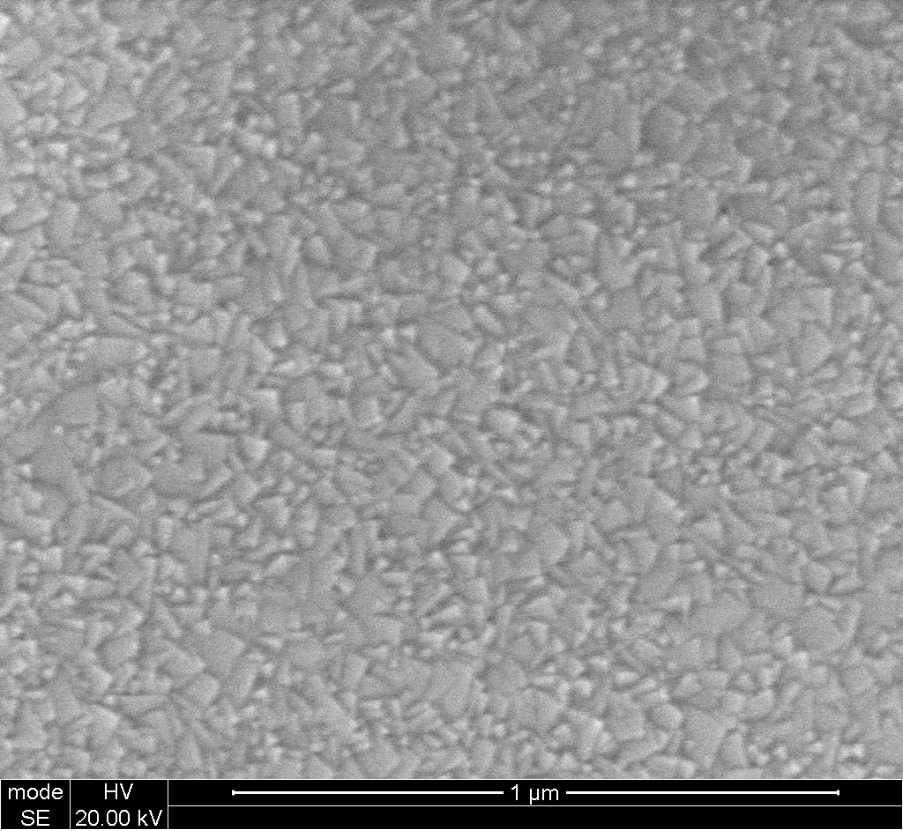
\includegraphics[width=.7\textwidth]{Figures/BZG-MgO-850-100000x-SE_019.pdf}
    \caption{Scanning electron microscopy image showing typical thin film microstructure of Gd:BaZrO$_3$ deposited on single crystalline MgO substrate by pulsed laser deposition.}
    \label{fig:films:sem:surface}
\end{figure}